\documentclass[crop,tikz]{standalone}% 'crop' is the default for v1.0, before it was 'preview'
\usepackage{tikz}
\usetikzlibrary{positioning,shapes.geometric,calc}
\usepackage{pgfplots} % loads tikz which loads pgf
\usepackage{xparse}
\pgfplotsset{compat=1.18}

\begin{document}
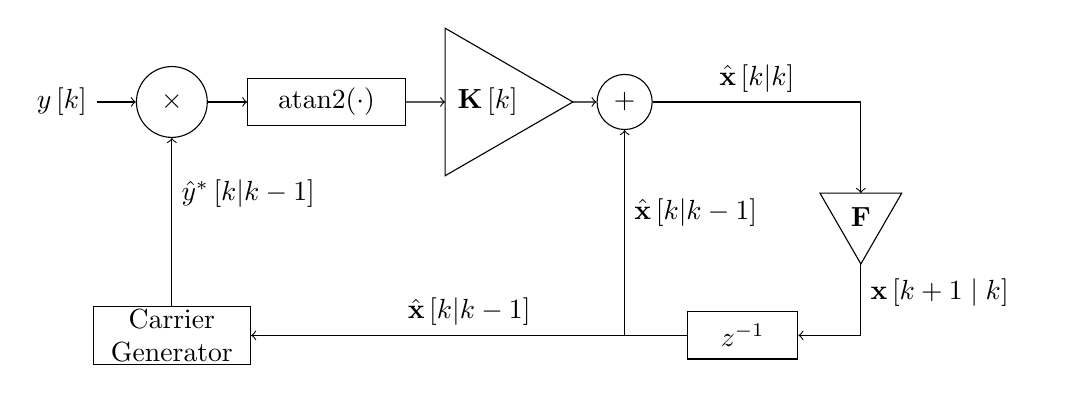
\begin{tikzpicture}
		% styles
		\tikzset{
			block/.style={draw, rectangle, minimum width=20mm, minimum height=6mm, align=center, inner sep=2pt, inner xsep=2pt, inner ysep=1pt},
			smallblock/.style={draw, rectangle, minimum width=14mm, minimum height=8mm, align=center, inner sep=0.5pt},
			smallblock/.style={draw, rectangle, minimum width=14mm, minimum height=6mm, align=center, inner sep=0.8pt, inner xsep=2pt, inner ysep=0.8pt},
			tri/.style={regular polygon, regular polygon sides=3, draw, minimum width=12mm, minimum height=8mm, align=center, inner sep=0pt, outer sep=0pt},
			sum/.style={circle, draw, minimum size=8mm, node distance=12mm, inner sep=0pt},
			sum/.style={circle, draw, minimum size=7mm, node distance=12mm, inner sep=0.8pt},
			mult/.style={circle, draw, minimum size=9mm, inner sep=0.8pt}
		}

		% nodes
		\node (in) at (0,0) {$y\left[ k \right]$};
		\node[mult, right=5mm of in] (mult) {$\times$};
		\node[block, right=5mm of mult] (atan) {atan2$(\cdot)$};
		\node[tri, right=5mm of atan, shape border rotate=-90] (K) {\(\mathbf{K}\left[ k \right]\)};
		\node[sum, right=3mm of K] (sum) {+};

		% feedback path (top to right)
		\node[tri, below=8mm of sum, shape border rotate=180, xshift=30mm] (F) {$\mathbf{F}$};
		\node[smallblock, below=6mm of F, xshift=-15mm] (z1) {$z^{-1}$};
		\node[right=28mm of z1] (dummy) {}; % spacer
        
        
		% connections
		\draw[->] (in) -- (mult);
		\draw[->] (mult) -- (atan); %node[midway, above] {$\tilde z\left[ k \right]$}
		\draw[->] (atan) -- (K);
		\draw[->] (K) -- (sum);
        
		\draw[->] (sum) -| (F) node[pos=0.25,above] {$\hat{\mathbf{x}} \left[ k|k \right]$};
		\draw[->] (F) |- (z1) node[pos=0.2, right] {\(\mathbf{x} \left[ k+1 \mid k \right]\)};
		\draw[->] (z1) -| (sum) node[pos=0.8,right] {$\hat{\mathbf{x}} \left[ k|k-1 \right]$};
        
		% bottom carrier generator placed at intersection of vertical through 'mult' and horizontal through 'z1'
		\node[block] (cg) at (mult |- z1) {Carrier\\Generator};
		\draw[->] (z1) -- (cg) node[pos=0.5,above] {$\hat{\mathbf{x}} \left[ k|k-1 \right]$};


		% bottom to Carrier Generator and up to multiplier
		% \draw[->] (xbpred) -| (cg) node[pos=0.25,below] {};
		\draw[->] (cg) -- ++(0,18mm) -| (mult) node[pos=0.5,right] {$\hat{y}^*\left[ k|k-1 \right]$};

		% prediction into sum
		% \draw[->] (xbpred) -- ++(24mm,0) |- (sum) node[pos=0.25,below] {$\hat x\left[ k|k-1 \right]$};

\end{tikzpicture}
\end{document}